\documentclass[12pt]{article}
\usepackage[utf8]{inputenc}
\usepackage[english]{babel}
\usepackage{a4wide}
\usepackage{graphicx}
\author{Lukáš Kerpl}
\title{Deska Use Case Diagrams}



\begin{document}

{\Huge \textbf{Deska}}

\vspace{0.2in}

{\large Tool for Central Administration of a Grid Site}

\vspace{0.5in}

{\large Use Case Diagrams}

\vspace{0.2in}

{\large Prepared for the Institute of Physics of the AS CR}

\vspace{0.2in}

{\large Version 1.0}

\vspace{0.2in}

{\large Date 2009-Nov-18}

\vspace{0.5in}

\tableofcontents

\newpage


\section{Purpose}
This document describes use cases of Deska, Tool for Central Administration
of a Grid Site. Use cases are devided into two parts. Grid managing, which
describes managing of the grid and has only one actor: Administrator.
The second part, Grid monitoring, describes monitoring of the grid and has
two actors: Administrator and Manager.

\section{Use cases}

\subsection{Grid managing}
This part describes managing of the grid and has only one actor: Administrator.

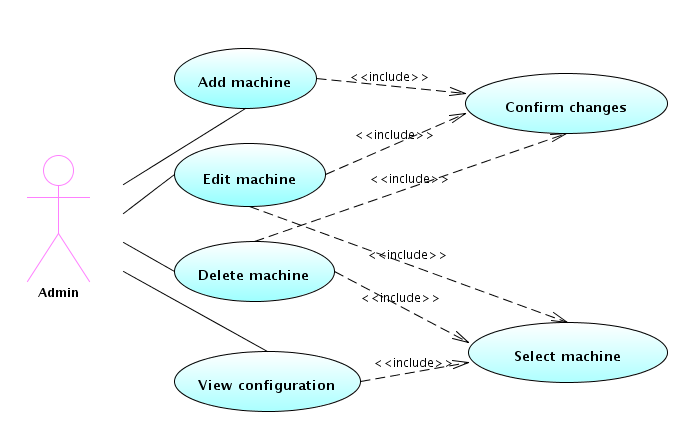
\includegraphics[width=\linewidth]{grid_managing.png}

\subsubsection{Select machine}
Select machine from the grid site.

Scenario:
\begin{itemize}
\item{System views list of all machines in the grid site}
\item{Administrator select one machine}
\end{itemize}

\subsubsection{Confirm changes}
Select machine from the grid site.

Scenario:
\begin{itemize}
\item{System views possible changes}
\item{Administrator checks and confirms this changes}
\item{System executes changes in configuration of the grid site}
\end{itemize}

\subsubsection{Add machine}
Add new machine into the grid site.

Scenario:
\begin{itemize}
\item{Administrator chooses, that he wants to add new machine}
\item{System views form to fill in}
\item{Administrator fills in this form}
\item{Include (confirm changes)}
\end{itemize}

\subsubsection{Edit machine}
Edit existing machine in the grid site.

Scenario:
\begin{itemize}
\item{Administrator chooses, that he wants to edit existing machine}
\item{Include (select machine)}
\item{System views form to fill in with appropriate values}
\item{Administrator makes changes in this form}
\item{Include (confirm changes)}
\end{itemize}

\subsubsection{Delete machine}
Delete machine from the grid site.

Scenario:
\begin{itemize}
\item{Administrator chooses, that he wants to delete existing machine}
\item{Include (select machine)}
\item{Include (confirm changes)}
\end{itemize}

\subsubsection{View configuration}
View configuration of machine from the grid site.

Scenario:
\begin{itemize}
\item{Administrator chooses, that he wants to see configuration of existing machine}
\item{Include (select machine)}
\item{System generates and view complete report from current configuration of the machine}
\end{itemize}

\subsection{Grid monitoring}
This part describes monitoring of the grid and has two actors: Administrator and Manager.

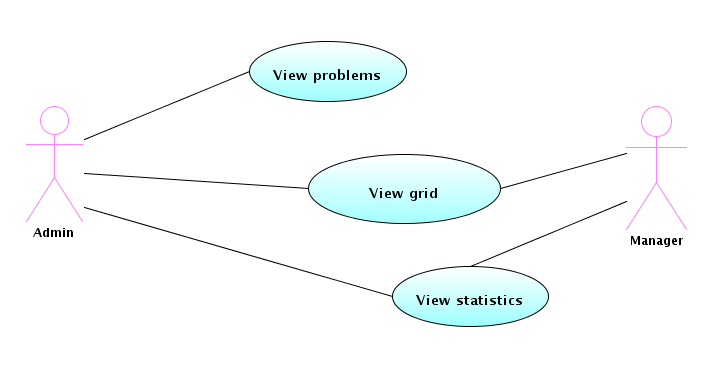
\includegraphics[width=\linewidth]{grid_monitoring.png}

\subsubsection{View problems}
View machines which indicates problems with describtion.

Scenario:
\begin{itemize}
\item{Administrator chooses, that he wants to see list of problematic machines}
\item{System views list of existing machines, which indicates problems and the description of the problems}
\item{Administrator can selects machine from the list and edit it's configuration}
\end{itemize}

\subsubsection{View grid}
View status of all machines in the grid site.

Scenario:
\begin{itemize}
\item{Administrator chooses, that he wants to see status of the grid site}
\item{System views status of all machines}
\end{itemize}

\subsubsection{View statistics}
View statistics from all machines in the grid site.

Scenario:
\begin{itemize}
\item{Administrator chooses, that he wants to see statistics of the grid site}
\item{ System views statistics of the grid site}
\end{itemize}

\section{Project Glossary}

Refer Tool for Central Administration of a Grid Site document.

\end{document}
